% ============================================================================
% ecvol-bench: identity-controlled benchmark for multimodal earnings-call
% volatility prediction (benchmark-first spine, DECISIONS 2026-08-26 S3).
% Condensed spine (2026-10-09); the 30-page long draft is tagged paper-long-2026-10-09.
%
% FORMAT: official ACL style (acl.sty + acl_natbib.bst from
% github.com/acl-org/acl-style-files, fetched 2026-10-09), as ARR requires.
%   [review]   anonymous, line numbers, page numbers  (ARR submission)
%   [preprint] names shown, page numbers, no line numbers
%   [final]    camera-ready
% The style loads geometry, caption, natbib and hyperref itself; do not load
% them again here.
% ============================================================================

\documentclass[11pt]{article}
\usepackage[review]{acl}

% --- Encoding & fonts (as in the ACL template) --------------------------------
\usepackage{times}
\usepackage{latexsym}
\usepackage[T1]{fontenc}
\usepackage[utf8]{inputenc}
\usepackage{microtype}
\usepackage{inconsolata}
\usepackage{xspace}

% --- Math, tables, graphics ---------------------------------------------------
\usepackage{amsmath}
\usepackage{amssymb}
\usepackage{booktabs}
\usepackage{graphicx}
\usepackage{multirow}
\usepackage{tikz}
\usetikzlibrary{positioning,calc,decorations.pathreplacing}
% The appendix \input{}s many table floats with little intervening text;
% raise the float-storage limit so they don't overflow ("Too many unprocessed floats").
\extrafloats{120}

% --- Bibliography: acl.sty sets \bibliographystyle{acl_natbib} itself; do not repeat it.

% --- Draft/TODO machinery -----------------------------------------------------
% Set \draftmode to false to hide TODOs for a clean render.
\newif\ifdraftmode\draftmodetrue
\newcommand{\TODO}[1]{%
  \ifdraftmode{\color{red!75!black}\textbf{[TODO:} #1\textbf{]}}\fi}
\newcommand{\pending}[1]{%
  \ifdraftmode{\color{orange!80!black}\textit{[pending: #1]}}\fi}

% --- Convenience macros -------------------------------------------------------
\newcommand{\ecvol}{\textsc{ecvol}\xspace}
% \ensuremath so these work both in text and inside an existing $...$ context.
\newcommand{\Rtwo}{\ensuremath{R^2_{\mathrm{OOS}}}\xspace}
\newcommand{\dv}{\ensuremath{\Delta v}\xspace}
\newcommand{\tickerdisjoint}{ticker-disjoint\xspace}

% ============================================================================
\title{\ecvol-bench: An Open, Identity-Controlled Benchmark for\
       Multimodal Earnings-Call Volatility Prediction}

% In [review] mode the style prints "Anonymous ACL submission" and ignores
% this block. Placeholder names show only with [preprint] or [final].
\author{First Author \
  Institution One \
  \texttt{first.author@example.edu} \And
  Second Author \
  Institution Two \
  \texttt{second.author@example.edu}}

% ============================================================================
\begin{document}
\maketitle
\begin{abstract}
% Condensed abstract (5-page spine, 2026-10-09). Every number traces to a
% manifested result CSV; see the header comment of each table in paper/tables/.
A decade of work predicts post-earnings-call stock volatility from call
transcripts and audio. We show that the evaluation substrate this literature
shares cannot support its claims: the canonical label and split files have a
zero-day embargo against 30-day targets, place 44--80\% of test calls' companies
in training, and anchor day~0 on the call date although the earnings release
precedes the open for most calls. We release \ecvol-bench, an open benchmark
over FinCall-Surprise and MAEC that repairs this: reconstructed company identity
and dates for a corpus that ships without them, EDGAR-measured release
timestamps, targets under both horizon conventions, embargoed and
\tickerdisjoint{} splits, econometric baselines, and an identity-control suite
that runs on any prediction file. Under these controls, modern frozen text and
audio representations add nothing to past volatility: adding either to a
past-volatility ridge lowers \Rtwo{} in all 16 split$\times$horizon cells, text
embeddings identify the company at 89.5\% probe accuracy, audio-only heads do no
better than a featureless intercept, and fusion beats HAR-RV in one horizon. Re-run on their
own data, the field's text models lose 12--82\% MSE when companies are held out
while price-based models do not move. Nothing degrades when the frozen pipeline
is scored on 475 calls held after every encoder's knowledge cutoff. All code,
metadata, splits, targets, features and result tables are released.

\end{abstract}

\section{Introduction}
\label{sec:intro}

An earnings call is the one regular occasion on which a company's managers speak
at length about their business. Since \citet{qin2019what}, a line of papers has
used both the transcript and the audio of these calls to predict how volatile the
stock will be over the following 3 to 30 trading days. HTML \citep{yang2020html},
MAEC \citep{li2020maec}, VolTAGE \citep{sawhney2020voltage}, DialogueGAT
\citep{sang2022dialoguegat}, KeFVP \citep{niu2023kefvp} and ECC Analyzer
\citep{cao2024ecc} all report beating classical forecasts. Two findings cast doubt
on that. \citet{scss2024} showed that transcript representations mostly tell the
model \emph{which company} is speaking, and that a simple forecast from the
company's own past volatility beats every transcript model. Across NLP, a
systematic review found that only 14\% of reported scores were reproduced
exactly \citep{belz2021repro}, and in financial NLP discontinued data APIs and
dead repository links make matters worse \citep{finnlp2025survey}.

We think both problems trace back to the same place. Nearly every paper in this
line is scored on one set of label and split files, handed down from paper to
paper. We audited those files (\S\ref{sec:substrate}). They leave no gap between
training and test dates even though each target runs 30 days past its call. Most
test calls come from companies that are also in training, and no paper reports
what happens when they are not. They define horizons in calendar days, which later
papers describe as trading days. They put day~0 on the date of the call, although
most companies publish their results before the market opens that day. The only
open corpus with raw audio, FinCall-Surprise \citep{fincall2025}, has no ticker,
date or speaker fields at all, so the checks that would expose the
company-identity problem cannot be run on it. Its successor, MM-FinEval
\citep{mmfineval2026}, adds tickers and dates but none of the checks.

\paragraph{What we contribute.}
(1)~\textbf{\ecvol-bench}, with company identities and dates recovered for
FinCall-Surprise (92.9\% of calls, and a 60-call manual audit passes 60/60),
release times from 8-K filings, three target families under both horizon
definitions, splits with a 30-session gap and company-disjoint splits, checksums
for every file, and a harness in which every table comes from one command
(\S\ref{sec:benchmark}). (2)~\textbf{An audit} of the shared label and split
files (Table~\ref{tab:substrate}). (3)~\textbf{Identity checks} (ticker probes,
same-company and random content swaps, company-disjoint evaluation), released as
a command that works on \emph{any} prediction file. (4)~\textbf{Results} for
modern open-weight text and audio models against strong baselines
(\S\ref{sec:results}). (5)~\textbf{A reproduction study} of the five runnable
models in this line, on their own data, with the same checks, plus a
code-availability audit of seventeen papers. (6)~\textbf{A post-cutoff test} of
the frozen pipeline on 475 calls from late 2025. Stages, checks and confirmatory
tests were recorded in a dated decision log, released with the benchmark, before
the corresponding results existed.

\paragraph{Related work.}
The design responds to known pitfalls. Company identity leaks into transcript
models \citep{scss2024}, and language models recover it even when names are
removed \citep{memorization2025}, so we add identity checks. Language models also
carry lookahead bias, and although diagnostics and cutoff-bounded models now exist
\citep{lookahead2025,datedgpt2026,lookaheadbench2026}, no earnings-call pipeline
had been scored on calls after its cutoff, so we do that. Persistence, GARCH and
HAR-RV \citep{corsi2009har} are hard to beat and often missing from comparisons
\citep{gukellyxiu2020}, so they anchor every table, and because audio features
encode speaker gender \citep{ama2024,emobias2024} we report that confound.
\citet{fastnumbers2026} time earnings releases from 8-K filings to predict
returns, but nobody had audited the volatility label sets. The strongest recent
positive results \citep{soundofrisk2025,cao2024ecc} report no identity checks and
release no code.

\section{The Substrate and the Benchmark}
\label{sec:benchmark}

\paragraph{The substrate the literature shares.}
\label{sec:substrate}
The EarningsCall (EC) benchmark of \citet{qin2019what} and the two MAEC cohorts
are scored on split and label files redistributed by VolTAGE and KeFVP. We
fetched them, manifested them by SHA-256 and audited them
(Table~\ref{tab:substrate}; \texttt{ecvol audit substrate}). The VolTAGE and
KeFVP test files are byte-identical: one physical label set, never recomputed
from prices. Every train/validation and validation/test boundary has a zero-day
gap (on EC, training ends and validation starts on 2017-08-03) against targets
that run 30 days past each call. On the temporal splits the field reports,
80.4\% (EC), 44.2\% (MAEC-15) and 55.7\% (MAEC-16) of test calls come from
companies also in training; a temporal split always permits this, but no paper in
the lineage reports the disjoint condition, so the confound of \citet{scss2024}
has never been measured on these benchmarks. The source paper defines its horizons
over \emph{calendar} days; most downstream work describes them as trading days,
which at $\tau{=}30$ is 21 versus 30 sessions. Finally, the shipped MAEC labels
correlate only 0.52--0.87 with calendar-day targets recomputed from prices under
the same call-date anchor (0.25--0.66 at $\tau{=}3$), so the lineage's labels are
not reproducible from prices under any single documented rule.

% Curated from data/results/result_table_5r.csv and result_table_5r_labels.csv
% (runs 20261006T202254Z / 20261006T202821Z-audit-substrate-48b9432a). Overlap = test calls whose
% ticker appears in train; embargo = calendar days between the last train (val)
% date and the first val (test) date. Ours = committed splits, same metrics.
\begin{table}[t]
\centering
\small
\begin{tabular}{lrrrrr}
\toprule
Benchmark / split & calls (tr/va/te) & overlap & embargo tr$\to$va & va$\to$te & label defect \\
\midrule
EC (Qin \& Yang)         & 392 / 56 / 112  & 80.4\% & 0 d & 0 d & 137 / 16{,}800 zero cells \\
MAEC-15 (KeFVP files)    & 535 / 76 / 154  & 44.2\% & 0 d & 0 d & 4 binary cols at $\tau$ \\
MAEC-16 (KeFVP files)    & 980 / 140 / 280 & 55.7\% & 0 d & 3 d & 4 binary cols at $\tau$ \\
\midrule
ours: FinCall temporal        & 1489 / 228 / 483 & 91.3\% & 47 d & 47 d & --- \\
ours: FinCall ticker-disjoint & 1706 / 243 / 484 & \textbf{0.0\%} & n/a & n/a & --- \\
ours: MAEC temporal           & 1666 / 69 / 529 & 79.4\% & 101 d & 48 d & --- \\
ours: MAEC ticker-disjoint    & 1884 / 271 / 533 & \textbf{0.0\%} & n/a & n/a & --- \\
ours: Earnings25 ticker-disjoint & 333 / 47 / 95 & \textbf{0.0\%} & n/a & n/a & --- \\
\bottomrule
\end{tabular}
\caption{\textbf{Substrate audit of the shared benchmark files} (Result Table 5R,
regenerated by \texttt{ecvol audit substrate} from SHA-256-manifested copies of the
VolTAGE and KeFVP repositories). The VolTAGE and KeFVP split files are
byte-identical. Overlap is a property every temporal split permits, ours included;
the point is that no paper in the lineage reports the disjoint condition. The
zero-day embargos leak 30-day target windows across every boundary. Shipped
MAEC labels join our calendar-day, call-date-anchored targets on 77--79\% of test calls at
$\tau\ge7$ and correlate 0.52--0.87 with them (0.25--0.66 at $\tau{=}3$).}
\label{tab:substrate}
\end{table}


\paragraph{Corpora and identity.}
\textbf{FinCall-Surprise} \citep{fincall2025} (primary; Apache-2.0; 2{,}688 calls,
2019--2021, MP3 audio, transcripts, slides) ships four fields per record and no
ticker, date, CIK or speaker names. We reconstruct identity and date from transcript
content and slide metadata, cross-check against prices, and release the table with
an 80-row manual override list: 2{,}496 calls resolve (92.9\%; 95.3\% of
earnings-type calls) and a 60-call manual audit passes 60/60. \textbf{MAEC}
\citep{li2020maec} (secondary; CC-BY-SA-4.0; $\sim$3{,}443 calls, 2015--2018,
sentence-aligned audio features, no raw audio) and \textbf{Earnings25}
\citep{jiang2026earnings25} (CC-BY-4.0; 514 S\&P~500 calls held July--December
2025, webcast MP3 at 64\,kbps for 281 calls and $\le$24\,kbps for 232) complete the
set; Earnings25 is post-cutoff for every model we use, and 475 of its calls resolve
to a constituent ticker and join prices.

\paragraph{Targets.}
Daily adjusted prices come from a free source cross-checked against Tiingo on 50
tickers. With $r_t$ the return on
session $t$ relative to day~0, the last session before the call's information is
public, the primary target is
$v_{\mathrm{post}}(\tau)=\ln\sqrt{\frac{1}{n}\sum_{t=1}^{n}(r_t-\bar r)^2}$ for
$\tau\in\{3,7,15,30\}$, with $v_{\mathrm{pre}}(\tau)$ defined over the sessions
ending at day~0. Under the \textbf{trading-day} convention $n=\tau$; under the
\textbf{calendar-day} convention of \citet{qin2019what} the window holds every
session within $\tau$ calendar days, so $n\approx0.7\tau$ (FinCall:
2.4/4.9/10.8/21.2 sessions) and at $\tau{=}3$ at most one session for a Thursday or
Friday call. Windows with fewer than two sessions are excluded with a reason code
(42.5\% of FinCall's calls at $\tau{=}3$ calendar days, for which the released label
sets still carry a value). The conventions are far from interchangeable:
$v_{\mathrm{post}}$ correlates 0.78 between them at $\tau{=}3$ and the persistence
MSE, the leaderboard's metric, is 44--63\% higher there under calendar days, so a
published MSE is uninformative unless its convention is stated (Appendix
Table~\ref{tab:convention}). Both ship as separate files; every result below uses
trading days, and the convention is a column of every result table. Two
identity-robust variants are added: the \textbf{change}
$\Delta v=v_{\mathrm{post}}-v_{\mathrm{pre}}$, which subtracts the company's own
level, and the \textbf{HAR-residual}. After joining, FinCall yields 2{,}433 calls
with a target (97.5\%) and MAEC 2{,}688 (78.6\%; 2015--2018 delistings).

\paragraph{Measured call timing.}
\label{sec:timing}
Fewer than 4\% of FinCall transcripts mention a clock time, so no call carries a
measured time of day. We take the information boundary from EDGAR: the acceptance
time of the earliest 8-K with Item~2.02 within three days before to one day after
the call date (89.3\% of FinCall, 68.6\% of MAEC, 99.8\% of Earnings25), with
recorded fallback tiers (Earnings25 call-start time, the before/after-market flag
of \citet{scss2024}, an after-hours assumption). A release before the open makes
the call date itself day~1. Against the
call-date anchor that every released label set uses, \textbf{day~0 moves for 53\%
of FinCall, 56\% of MAEC and 72\% of Earnings25 calls}, almost always one session
earlier: under the published anchor the reaction session sits in the \emph{pre}
window for most of the corpus. On the measured anchor the persistence MSE is up to
11\% higher on FinCall, 25\% on MAEC and 27\% on Earnings25, and because the
reaction session now enters the post window, $\Delta v$ acquires a positive mean
(FinCall $+0.52$ at $\tau{=}3$, $+0.10$ at $\tau{=}30$). The call-date targets are
shipped as a labelled variant for comparison with prior label sets.

\paragraph{Splits and release.}
\emph{Temporal} splits ($\sim$70/10/20, calendar order) carry a 30-trading-day
embargo so that no target window crosses a boundary; \emph{\tickerdisjoint} splits
(grouped, seeded) put no validation or test company in training (overlap 0.0\%,
against 91.3\% FinCall and 79.4\% MAEC on our own temporal splits); a
\emph{combined} split enforces both. Every feature function receives an
\texttt{as\_of} timestamp and the harness fails any feature that reads later price
data; leakage assertions run in CI. The release contains every artefact above, the
derived-feature archives, the harness, and every result CSV with its run manifest
(resolved config, git SHA, seeds, file hash); raw audio and transcripts are never
redistributed.

\section{Models, Protocol and Checks}
\label{sec:setup}

\paragraph{Models, from simplest to richest.}
We organise our own models in stages. \textbf{Stage 0} holds the classical
forecasts: persistence ($\hat v=v_{\mathrm{pre}}$), the training-set mean of the
target (a constant), EWMA ($\lambda{=}0.94$), HAR-RV \citep{corsi2009har} and
GARCH(1,1). \textbf{Stage 1} is a LightGBM model on past-volatility features,
transcript length, number of Q\&A turns and a \textbf{company fixed effect}, our
identity-only baseline. \textbf{Stage 2} uses the transcript: BGE-M3
\citep{bge2024} embeddings pooled per section (1024-d), FinBERT \citep{finbert}
sentiment aggregates and surface statistics. \textbf{Stage 3} uses the audio, resampled to
16\,kHz mono: eGeMAPSv02 functionals \citep{opensmile}, and WavLM-Large
\citep{wavlm} and emotion2vec+ \citep{emotion2vec} embeddings over 30-second
windows, averaged per call. \textbf{Stage 4} combines modalities by gated fusion or by
stacking (a ridge over the text, audio and Stage-1 predictions, fit on the
validation set). From Stage~2 on, every model is reported with and without a block
of past-volatility features ($v_{\mathrm{pre}}$ at all horizons plus the HAR-RV
inputs). The prediction heads are a ridge regression, with its penalty chosen on
validation, and a small MLP run with five seeds. The MLPs are unstable across seeds
(standard deviation of \Rtwo{} up to 6.8), so the main grid uses one deterministic
model per stage, chosen before the results were known; MLP cells are in
Appendix~\ref{app:complete}.

\paragraph{Metrics and tests.}
We report MSE on log realised volatility and, as the headline metric, \Rtwo{}
relative to persistence \citep{gukellyxiu2020}, defined as
$1-\sum(y-\hat y)^2/\sum(y-\hat y_{\mathrm{persist}})^2$. Because $\Delta v$ has a
positive mean on the measured anchor, persistence (which predicts $\Delta v{=}0$)
is a weak reference there, so every $\Delta v$ claim is also compared with the
constant model. Diebold--Mariano tests \citep{dm1995} with the small-sample
correction compare per-call squared errors against persistence and against the
previous stage. The confirmatory comparisons (each stage against Stage~1 on
$\Delta v$ across horizons, Stage~4 against the best single modality, and the
published split against the controlled split for each reproduced model) are
Holm-corrected; all other analyses are exploratory.

\paragraph{Identity checks.}
\label{sec:controls}
We use four. (1)~A \emph{company-only} model predicts each company's training
mean. (2)~A \emph{same-company swap} gives each test call the transcript or audio
of another call by the same company, and a \emph{random swap} gives it any other
call. A model that does not change under the first is reading identity; one that
does not change under the second is reading nothing. (3)~A linear \emph{probe}
tries to recover the ticker from the frozen call embedding. (4)~Every table shows
\tickerdisjoint{} results next to temporal ones. The command
\texttt{ecvol audit predictions} runs the prediction-side versions of these
checks, plus split integrity, seen-versus-unseen companies, the between-company
share of prediction variance and company-clustered significance, on any file with
one row per (call, ticker, date, split, horizon, truth, prediction), so a published
result can be checked from the one file its authors already have.

\paragraph{Reproductions and post-cutoff tests.}
Of seventeen papers in this line, one releases code that runs as released
(Same-Company-Same-Signal), seven release code that needs repairs or inputs that
were never shipped, and nine release nothing usable (Table~\ref{tab:code-audit}).
We rerun the five with usable code (HTML, KeFVP, Same-Company-Same-Signal,
\citealp{sawhney2020mm}, DialogueGAT) \emph{on their own data}, using the authors'
code wherever it can be made to start and a line-by-line port where it cannot
(every patch is in a released ledger), first against the published number
and then under a gapped split and a \tickerdisjoint{} split of the same data.
Earnings25 allows two more tests: the frozen Stage-3 audio models rerun by
bitrate, and the whole FinCall-trained pipeline scored, with no retraining, on
calls that postdate every model's training cutoff.

\section{Results}
\label{sec:results}

Headline tables use FinCall-Surprise, the identity-robust $\Delta v$ target and
the trading-day convention; MAEC, level-$v$, MSE, both conventions and every head
are in Appendix~\ref{app:complete}, regenerated byte-identically by
\texttt{ecvol report} from manifested CSVs.

% Generated by make_main_tables.py from data/results/result_table_{1,2,4,8}.csv.
\begin{table}[t]
\centering
\footnotesize
\setlength{\tabcolsep}{2.5pt}
\begin{tabular}{lrrrr}
\toprule
Model & $\tau$=3 & $\tau$=7 & $\tau$=15 & $\tau$=30 \\
\midrule
\multicolumn{5}{l}{\textit{Temporal split ($n{=}483$)}}\\
S0 train mean & 0.165 & 0.158 & 0.060 & 0.088 \\
S0 HAR-RV & 0.444 & 0.372 & 0.138 & $-$0.285 \\
S0$'$ past-vol ridge & 0.412 & 0.314 & 0.094 & 0.113 \\
S1 GBDT (ticker FE) & 0.340 & 0.249 & $-$0.126 & $-$0.948 \\
S2 text ridge + vol & 0.333\dag & 0.285 & 0.080 & $-$0.077\dag \\
S3 audio ridge + vol & 0.353\dag & 0.268\dag & 0.033\dag & 0.050\dag \\
S4 stack fusion & 0.406 & 0.347 & 0.066 & 0.100 \\
\midrule
\multicolumn{5}{l}{\textit{Date-ordered disjoint split ($n{=}97$)}}\\
S0 train mean & 0.152 & 0.147 & 0.080 & 0.119 \\
S0 HAR-RV & 0.446 & 0.384 & 0.209 & $-$0.120 \\
S0$'$ past-vol ridge & 0.409 & 0.315 & 0.159 & 0.158 \\
S1 GBDT (ticker FE) & 0.300 & 0.047 & $-$0.324 & $-$1.063 \\
S2 text ridge + vol & 0.160\dag & 0.169\dag & 0.039\dag & $-$0.056\dag \\
S3 audio ridge + vol & 0.312\dag & 0.147\dag & 0.057\dag & 0.098 \\
S4 stack fusion & 0.339\dag & 0.108\dag & $-$0.180\dag & $-$0.028\dag \\
\bottomrule
\end{tabular}
\caption{\textbf{The ladder on FinCall-Surprise.} \Rtwo{} vs.\ persistence on
$\Delta v$ (test). Persistence is 0 by construction. The second block keeps test
companies out of training and the split in date order. One
canonical model per stage (the Stage-3 ridge uses WavLM and eGeMAPS). Each
content cell is tested against the
past-volatility ridge S0$'$ on the same calls. A dagger marks a 95\% interval of
the relative MSE reduction, resampled by company, that lies below the
2\% margin fixed in advance, an asterisk one that lies above it, and an unmarked
cell is inconclusive (Appendix Table~\ref{tab:increment}). The full grid, MAEC,
level-$v$, MSE and the MLP heads are in Appendix~\ref{app:complete}.}
\label{tab:grid}
\end{table}


\paragraph{The floor.}
Table~\ref{tab:grid} sets it. HAR-RV is strong except in one cell: on the FinCall
temporal split at $\tau{=}30$ the training window is COVID-inflated and the test
year (2021) is calm, so every long-horizon level forecast, ours and every content
head, falls below persistence (level-$v$: HAR $-0.29$, text $-0.45$, audio $-0.76$,
fusion $-0.23$). The same models pass on the
\tickerdisjoint{} split and on MAEC (a documented regime exception). Because the
reaction session enters the post window on the measured
anchor, a featureless train-mean intercept already reaches 0.17/0.16/0.06/0.09
(temporal) and 0.20/0.20/0.13/0.04 (\tickerdisjoint), the reference for every
$\Delta v$ claim below.

\paragraph{Text reads identity (Table~\ref{tab:controls}).}
The text-only ridge head sits at the intercept: 0.18/0.20/0.04/$-$0.13 (temporal)
and 0.20/0.22/0.20/0.17 (\tickerdisjoint), never within 0.09 of HAR-RV; the MLP
heads overfit. Adding text to the past-volatility ridge \emph{lowers} \Rtwo{} in all
eight cells. A linear probe
recovers the ticker from the frozen call embedding at 89.5\% on FinCall and 53.9\%
on MAEC. On the temporal split, where test companies recur in training, giving each
test call the transcript of \emph{another call of the same company} changes the head
by at most 0.02 while a global shuffle degrades it: the head reads which company is
speaking. On the \tickerdisjoint{} split the same-company swap does cost the head at
$\tau\ge15$, so some call-specific signal exists in unseen companies, but it lies
below the past-volatility floor and vanishes once that block is present (text$+$vol
0.301 vs.\ past-vol 0.318 at $\tau{=}30$). MAEC repeats the pattern.

% Generated by make_main_tables.py from four controls CSVs.
\begin{table}[t]
\centering
\scriptsize
\setlength{\tabcolsep}{3pt}
\begin{tabular}{lrr}
\toprule
Identity probe (linear, frozen call embedding) & accuracy & $\times$chance \\
\midrule
BGE-M3 text, FinCall (357 tickers) & 89.5\% & 319$\times$ \\
BGE-M3 text, MAEC (902 tickers) & 53.9\% & 487$\times$ \\
WavLM audio, FinCall (356 tickers) & 76.3\% & 271$\times$ \\
emotion2vec+ audio, FinCall (356 tickers) & 29.4\% & 105$\times$ \\
\bottomrule
\end{tabular}

\vspace{0.2em}
\begin{tabular}{lrrrr}
\toprule
Content swap (\Rtwo{} on $\Delta v$) & $\tau$=3 & $\tau$=7 & $\tau$=15 & $\tau$=30 \\
\midrule
\multicolumn{5}{l}{\textit{Text ridge, temporal split}}\\
\quad real & 0.182 & 0.202 & 0.044 & $-$0.133 \\
\quad same-company swap & 0.174 & 0.194 & 0.047 & $-$0.110 \\
\quad random swap & 0.145 & 0.110 & 0.008 & $-$0.152 \\
\multicolumn{5}{l}{\textit{Text ridge, date-ordered company-disjoint}}\\
\quad real & 0.122 & 0.133 & 0.009 & $-$0.092 \\
\quad same-company swap & 0.136 & 0.139 & 0.019 & $-$0.057 \\
\quad random swap & 0.173 & 0.166 & 0.084 & 0.099 \\
\bottomrule
\end{tabular}
\caption{\textbf{Identity checks.} Frozen embeddings identify the company far
above chance. Where companies recur (temporal), giving a test call another call
by the \emph{same} company barely changes the text model, while a random call
hurts. On the date-ordered company-disjoint split the real transcript scores no
better than either swap. The audio swaps are in Appendix Table~\ref{tab:audio}.}
\label{tab:controls}
\end{table}


\paragraph{Audio is inert beyond past volatility.}
Audio-only ridge heads on eGeMAPS, WavLM-Large and emotion2vec+ sit within 0.10 of
the train-mean intercept at every horizon on both splits and never above it by more
than 0.02 (temporal WavLM 0.156/0.148/$-$0.027/$-$0.008 against
0.165/0.158/0.060/0.088). Adding WavLM to the past-volatility ridge lowers \Rtwo{} in
all eight cells. The audio-shuffle control (Table~\ref{tab:controls}, bottom) shows
the past-vol-augmented head keeping its score when every test call receives a
\emph{random other company's} audio at $\tau{=}3$ (0.456 $\to$ 0.453); at longer
horizons the shuffle costs more, but the real-audio head is still below the
past-vol-only ridge, so what audio contributes does not add to past volatility. Identity is nonetheless encoded: a probe recovers
the ticker from pooled WavLM embeddings at 76.3\%. An exploratory gender check
(dominant-speaker F0 proxy) finds per-group test MSE of 0.243 vs.\ 0.239. Re-run
on Earnings25 by bitrate
(one call per company, so the global shuffle is the control), the audio increment
(real minus shuffled \Rtwo) never exceeds 0.03, is negative in 7 of 12 stratum
cells, and the 64\,kbps stratum is not the better one (Appendix
Table~\ref{tab:earnings25-audio}): the FinCall result is not an artefact of its
40\,kbps transcodes.

\paragraph{Fusion.}
Gated fusion is worse than its inputs everywhere. The late-fusion stack is the best
content stage but stays below HAR-RV in six of eight cells; it exceeds HAR-RV only
in the regime cell (0.100 vs.\ $-$0.285, still below the past-vol ridge at 0.113)
and at \tickerdisjoint{} $\tau{=}30$ (0.396 vs.\ 0.345; Holm $p{=}0.003$ vs.\
Stage~1, no pre-registered test vs.\ HAR-RV). The stack beats the text and audio
stages in seven of eight cells but not the past-volatility stage, so multimodal is
not better than the best unimodal model once past volatility is that model, and the
pre-registered positive-framing gate (content gains
surviving the controls on at least two of four horizons) was missed at Stages~2, 3
and~4, as the decision log records.

\paragraph{The field's own models (Table~\ref{tab:repro-main}).}
Of the five runnable papers, the results that reproduce are those of price-only or
same-company models (Appendix~\ref{app:repro}). Same-Company-Same-Signal
reproduces from the shipped data: TSMixer to $10^{-5}$, TMLP within 0.02 including
the paper's finding that embeddings shuffled within a company do as well as the real
ones, and its training-free augmented same-company history lands within 0.05 of
KeFVP's published MSE at every horizon on EC and MAEC-15 with no text and no
training, a model with no definition once companies are held out. KeFVP, a price
series conditioned on text whose audio branch is disabled in its own code,
reproduces seven of eight MAEC cells within one published standard deviation after
six import-level repairs; its EC row, run without the unavailable knowledge-enhanced
embeddings, sits above all four published cells and is not counted. HTML's released
driver splits features and labels with independent unseeded shuffles, so it cannot
have produced the published table; with the authors' model classes verbatim the
published recipe underfits at every horizon $\ge15$ on every split. The published
ensemble of \citet{sawhney2020mm} is reachable only because untrained text and
audio branches act as an intercept on a finance SVR whose mixing weights the code
tunes on the test set. DialogueGAT's corpus was never released. Under our controls
(Table~\ref{tab:repro-main}), holding companies out costs the three text models
12--82\% MSE while TSMixer and KeFVP do not move, with training sets as large (EC)
or reduced by the same third (DEC, MAEC); the embargo moves models by at most 13\%;
and HTML's own trained model changes by at most 4\% when a test transcript is swapped
for another call of the same company (under 1\% on the \tickerdisjoint{} split)
against 9--23\% for a different company's call. What HTML reads from a transcript is
which company is speaking.

% Generated by make_main_tables.py from the values in tables/repro_controls.tex.
\begin{table}[t]
\centering
\scriptsize
\setlength{\tabcolsep}{3pt}
\begin{tabular}{lrrrr}
\toprule
Model (data), change in test MSE & $\tau$=3 & $\tau$=7 & $\tau$=15 & $\tau$=30 \\
\midrule
\multicolumn{5}{l}{\textit{Companies held out (\tickerdisjoint{} vs.\ the model's own split)}}\\
HTML text (EC) & +18\% & +55\% & +55\% & +82\% \\
HTML text$+$audio (EC) & +20\% & +44\% & +61\% & +70\% \\
Sawhney ensemble (EC) & +13\% & +28\% & +41\% & +38\% \\
SCSS TMLP, text (DEC) & +12\% & +23\% & +25\% & +27\% \\
SCSS TSMixer, price (DEC) & +7\% & +5\% & $-$6\% & $-$8\% \\
KeFVP, text$+$price (MAEC-15) & $-$3\% & +4\% & +3\% & $-$1\% \\
KeFVP, text$+$price (MAEC-16) & $-$9\% & $-$3\% & $-$10\% & $-$4\% \\
\midrule
\multicolumn{5}{l}{\textit{30-session embargo vs.\ the model's own split}}\\
HTML text (EC) & +10\% & +3\% & $-$3\% & +11\% \\
Sawhney ensemble (EC) & +5\% & $-$6\% & $-$2\% & $-$9\% \\
SCSS TMLP (DEC) & $-$4\% & +1\% & 0\% & +3\% \\
\midrule
\multicolumn{5}{l}{\textit{HTML text, transcript replaced by (own split, 97 calls)}}\\
another call, \emph{same} company & +1\% & +4\% & +3\% & +2\% \\
a call of a \emph{different} company & +9\% & +11\% & +21\% & +23\% \\
\bottomrule
\end{tabular}
\caption{\textbf{The field's runnable models under our controls} (Result
Table~6R-C). Each row keeps the configuration of Appendix Table~\ref{tab:faithful}
and changes only the split. Holding companies out costs every text model 12--82\%
and leaves the price-dominated models unchanged, with held-out training sets as
large (EC) or cut by the same third (DEC, MAEC). Absolute values are in Appendix
Table~\ref{tab:repro-controls}.}
\label{tab:repro-main}
\end{table}


\paragraph{Post-cutoff (Table~\ref{tab:lookahead}).}
Scored unchanged on 475 Earnings25 calls from late 2025, after the training cutoff
of every encoder and on companies none of the heads has seen, no head that was
competitive in-cutoff degrades on level-$v$: HAR-RV rises from 0.44/0.37/0.14/$-$0.29 to
0.60/0.54/0.35/0.08 and the content ridges rise with it (the 3k-dimensional fusion
ridge is unstable at $\tau{=}30$). Levels are not comparable
across the cutoff (different years and universes); the ordering is, and it survives:
HAR-RV beats every content head at every horizon, and no content head that was
competitive in-cutoff collapses post-cutoff. Under the call-date anchor of the published label sets the same frozen heads
collapse in-cutoff (text$+$vol on $\Delta v$: $-1.7$ to $-3.6$; Appendix
Table~\ref{tab:lookahead-assumed}), because the learned past-volatility block absorbs
the reaction session that the after-hours rule leaves in the pre-window.

% Generated by make_main_tables.py from data/results/result_table_7.csv.
% Level-v target, R^2_OOS vs persistence; in = FinCall temporal test (2021, in-cutoff),
% post = 475 Earnings25 calls (Jul-Dec 2025), same frozen heads, no retraining.
\begin{table}[t]
\centering
\scriptsize
\setlength{\tabcolsep}{2.5pt}
\begin{tabular}{lrrrr}
\toprule
Head (in-cutoff $\to$ post-cutoff) & $\tau$=3 & $\tau$=7 & $\tau$=15 & $\tau$=30 \\
\midrule
S0 train mean & 0.36$\to$0.58 & 0.14$\to$0.47 & $-$0.37$\to$0.15 & $-$1.05$\to$$-$0.29 \\
S0 HAR-RV & 0.44$\to$0.60 & 0.37$\to$0.54 & 0.14$\to$0.35 & $-$0.29$\to$0.08 \\
S2 text ridge + vol & 0.43$\to$0.57 & 0.34$\to$0.50 & 0.03$\to$0.25 & $-$0.45$\to$$-$0.20 \\
S3 WavLM ridge + vol & 0.38$\to$0.57 & 0.24$\to$0.43 & $-$0.09$\to$0.15 & $-$0.66$\to$$-$0.32 \\
S4 fusion ridge + vol & 0.41$\to$0.50 & 0.32$\to$0.46 & $-$0.02$\to$0.20 & $-$0.63$\to$$-$1.93 \\
\bottomrule
\end{tabular}
\caption{\textbf{Frozen-pipeline post-cutoff evaluation} (Result Table~7).
Heads fit once on FinCall's training split, scored unchanged in-cutoff (the 2021
FinCall test year) and post-cutoff (475 Earnings25 calls, late 2025); level-$v$,
\Rtwo{} vs.\ persistence. No head competitive in-cutoff degrades; the ordering survives, with
HAR-RV above every content head at every horizon. Month-cluster bootstrap CIs and
$\Delta v$ rows are in the released CSV.}
\label{tab:lookahead}
\end{table}


\section{Discussion and Conclusion}
\label{sec:discussion}

Four things hold across the whole set of models. Classical volatility forecasts
are hard to beat, and measuring against persistence exposes a regime failure that
raw MSE hides. Text features add nothing to past volatility, and we can see why:
the embeddings identify the company, and where companies recur in training,
swapping in another call by the same company changes nothing. Audio features add
nothing either, at 40\,kbps or 64\,kbps, even though they too identify the
company, and combining them does not help. None of this could be seen
with the files the field has been using, and the same checks on the field's own
code and data give the same answer: what reproduces is price-only models or
same-company history, and the text models lose their edge as soon as the company
is new. The strongest recent positive results \citep{soundofrisk2025,cao2024ecc}
report no identity checks and release no code; \texttt{audit predictions} makes
the check cheap. We do not claim that transcripts and audio carry no information
about a company's risk. We claim that the benchmarks in use cannot tell that
information apart from knowing which company is speaking, and that once they can,
nothing yet built beats a forecast from past volatility.

\section{Recommendations and Outlook}
\label{sec:recommendations}

The results above are not an argument against using earnings calls. They are an
argument about what an evaluation has to control for before a content effect can
be claimed. We suggest that future work on this task report, at minimum:
(1)~a \textbf{company-disjoint} split next to the temporal one, since identity
carries most of the apparent signal; (2)~a \textbf{gap} of at least the longest
horizon between training and test dates; (3)~\textbf{past-volatility baselines}
(persistence, HAR-RV) and, on change targets, a constant, as the reference for
every claim; (4)~the \textbf{same-company and random swaps} or the released
audit command, so that a gain can be attributed to the call rather than to the
company; (5)~\textbf{day~0 measured} from the release time rather than the call
date; and (6)~the \textbf{horizon definition} (calendar or trading days) stated
with every number. \ecvol-bench provides each of these for FinCall-Surprise and
MAEC, and the audit command applies the checks to any prediction file.

There is also reason to expect that content signal can be found once it is
looked for in the right place. Measured release times make
\textbf{event-window targets} possible, such as the volatility of the first
sessions after the release, where language about guidance and surprise should
matter most and where same-company history explains least. \textbf{Structured
features} extracted from the call, such as guidance changes and the gap between
the quantitative surprise and management's framing of it, can be audited one
field at a time, in contrast to pooled embeddings, and can be combined with the
fast numeric signal that \citet{fastnumbers2026} show arrives first.
\textbf{Audio} has so far been tested only on lossy webcast transcodes without
speaker diarisation; recordings at source quality with resolved speakers are the
fair test of prosody. \textbf{Larger company-disjoint corpora} are now within
reach, since MM-FinEval \citep{mmfineval2026} ships ticker and date fields and the
checks here transfer to it directly. Each of these can be evaluated against the
released baselines on the first day, which is what the benchmark is for.


% ACL unnumbered sections (not counted toward the page limit)
\section*{Limitations}
\addcontentsline{toc}{section}{Limitations}

\textbf{One post-cutoff quarter.} The post-cutoff test rests on 475 calls from a
single calm quarter and a different universe from the training corpus, so it
bounds contamination in the ordering of models, not in their absolute scores.
\textbf{Reproductions run on their own data}, not on \ecvol-bench, to keep ``the
model fails'' separable from ``the model does not transfer''. Two carry known
costs. KeFVP's released EC embeddings are unavailable upstream, and DialogueGAT's
corpus was never released, so our port stops at its protocol. \textbf{MLP heads
are seed-unstable} (standard deviation of \Rtwo{} across seeds up to 6.8 on the
level target and 1.1 on $\Delta v$), which is why the grid uses deterministic
models. MLP cells in the appendix are seed means with that caveat.
\textbf{Short-horizon \Rtwo{} inflation.} The persistence denominator is noisiest
at $\tau{=}3$ (its MSE is about 2.8 times that at $\tau{=}7$), so short-horizon
gains are easier to show. \textbf{Timestamps.} 10.7\% of FinCall and 31.4\% of
MAEC calls (13.0\% of the MAEC calls that carry targets) have no Item~2.02 filing
in the window and use a recorded fallback tier, and intraday releases are treated
as after-hours. Results under the
call-date anchor of prior label sets are not interchangeable with ours, and the
call-date targets are shipped as a variant. \textbf{Regime sensitivity.}
FinCall-Surprise spans COVID. The temporal $\tau{=}30$ failure shows that
long-horizon level forecasts are regime-sensitive, which is why we emphasise
$\Delta v$ and per-year breakdowns. \textbf{MAEC coverage.} Its 78.6\% price-join
rate (2015--2018 delistings) makes it a secondary corpus, and it ships no raw
audio. \textbf{Source audio.} Every FinCall file is a 40\,kbps MP3 transcode and
Earnings25 is 64\,kbps or lower, so no result here is established on lossless
audio. \textbf{No diarisation.} Audio is pooled per call, and the gender analysis
uses a dominant-speaker pitch proxy. \textbf{Identity reconstruction is
imperfect.} 7.1\% of FinCall calls remain unresolved and are excluded with a
reason code.

\section*{Ethical Considerations}
\addcontentsline{toc}{section}{Ethical Considerations}

\textbf{Data and licensing.} We use openly licensed corpora (FinCall-Surprise
under Apache-2.0, MAEC under CC-BY-SA-4.0, Earnings25 under CC-BY-4.0) and
open-weight models. Derived features inherit and state their upstream licence, and
raw audio or transcripts from sources with unclear terms (EC, DEC, the reproduced
repositories) are never redistributed. Calls are public corporate disclosures, and
we release no speaker-level audio or identity, only pooled per-call features.
\textbf{Gender confound.} Audio features encode speaker gender and female
executives are underrepresented in these corpora
\citep{ama2024,emobias2024,docfin2022}, so we report a gender-confound diagnostic
rather than silently propagate the bias. \textbf{Intended use.} This is a
forecasting-research benchmark, not investment advice. Predictions are noisy and
regime-sensitive and should not drive automated trading.
\textbf{Reproducibility.} Given the documented reproducibility problems in
financial NLP \citep{finnlp2025survey}, the environment is pinned, every data file is
checksummed, every result CSV regenerates byte for byte from its command and run
manifest, and the curated tables copy cells from those CSVs.


\bibliography{refs}

\appendix
\section{Extended Results}
\label{app:complete}

This appendix holds the full set of models behind each main-text table, the
horizon-definition comparison, the reproduction study in detail, the Earnings25
bitrate study, the call-date-anchor variant of the post-cutoff test, and the
code-availability audit. The complete generated grids (Result Tables 1--4, every
corpus, target, metric, split and horizon) are in the separate supplement. Every
number traces to a released result CSV with a run record, and the curated tables
copy cells from those CSVs (\texttt{REPRODUCE.md} lists the command behind each).

% Stage-ladder schematic (Stage 0 -> 4, plus the reproduction track).
\begin{figure}[t]
\centering
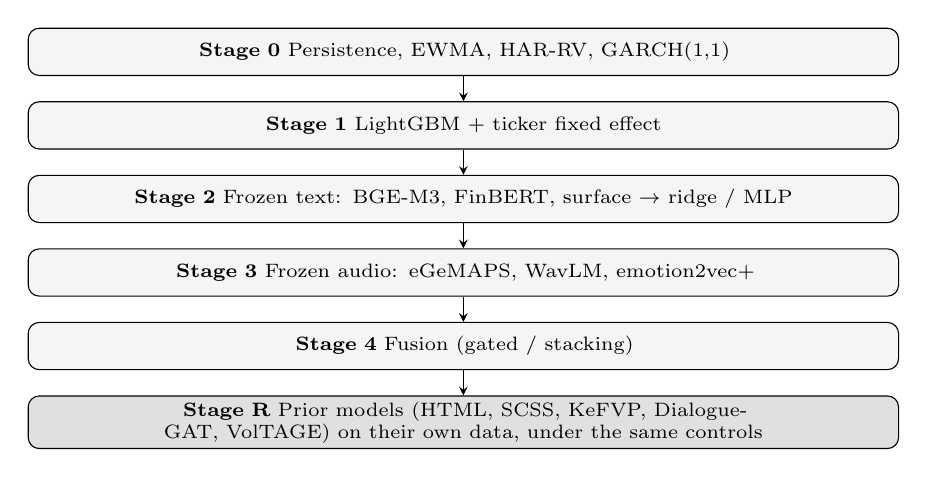
\begin{tikzpicture}[
    node distance=3.2mm,
    box/.style={draw, rounded corners, align=center, font=\scriptsize,
                inner sep=2pt, text width=0.9\linewidth, minimum height=6mm},
    stage/.style={box, fill=black!4},
    repro/.style={box, fill=black!12},
]
\node[stage] (s0) {\textbf{Stage 0} Persistence, EWMA, HAR-RV, GARCH(1,1)};
\node[stage, below=of s0] (s1) {\textbf{Stage 1} LightGBM $+$ ticker fixed effect};
\node[stage, below=of s1] (s2) {\textbf{Stage 2} Frozen text: BGE-M3, FinBERT, surface $\to$ ridge / MLP};
\node[stage, below=of s2] (s3) {\textbf{Stage 3} Frozen audio: eGeMAPS, WavLM, emotion2vec+};
\node[stage, below=of s3] (s4) {\textbf{Stage 4} Fusion (gated / stacking)};
\node[repro, below=of s4] (sr) {\textbf{Stage R} Prior models (HTML, SCSS, KeFVP, DialogueGAT, VolTAGE) on their own data, under the same controls};
\foreach \a/\b in {s0/s1, s1/s2, s2/s3, s3/s4, s4/sr}
  \draw[->, >=stealth] (\a) -- (\b);
\end{tikzpicture}
\caption{\textbf{The modelling ladder.} From Stage~2 up, every model also carries
past-volatility covariates (and is reported with them ablated). Every stage runs
through the identity checks. The darker box is the reproduction track, which
applies the same checks to published models on their own data.}
\label{fig:pipeline}
\end{figure}


\subsection{Stages 0--3: all models}
Tables~\ref{tab:baselines}, \ref{tab:text} and~\ref{tab:audio} give the full
Stage-0/1, Stage-2 and Stage-3 model sets on the $\Delta v$ target, including the
past-volatility-only and MLP heads omitted from Table~\ref{tab:grid}.

Figure~\ref{fig:ladder} plots the canonical model of each stage from
Table~\ref{tab:grid} against the train-mean constant.

\begin{figure*}[t]
\centering
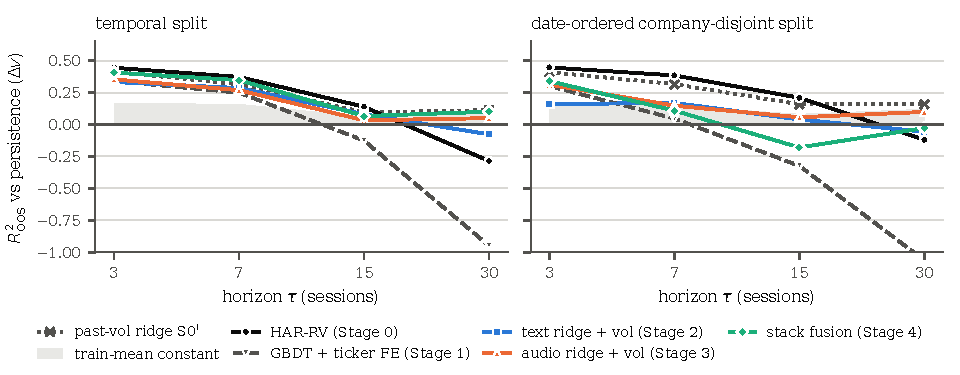
\includegraphics[width=\textwidth]{figures/fig_ladder.pdf}
\caption{\textbf{The ladder.} \Rtwo{} vs.\ persistence on $\Delta v$ (FinCall
test) for the canonical model of each stage; the shaded band is the train-mean
constant. No content stage clears HAR-RV on the temporal split, and on the
\tickerdisjoint{} split only the fusion stack does, at $\tau{=}30$. Data:
Table~\ref{tab:grid}.}
\label{fig:ladder}
\end{figure*}

% Curated headline: Stage-0/1 baselines, FinCall, Delta-v target, R^2_OOS vs
% persistence (test). Values copied from data/results/result_table_1.tex
% (temporal n=483; ticker-disjoint n=484). * = DM-significant vs persistence.
\begin{table}[t]
\centering
\small
\setlength{\tabcolsep}{4pt}
\begin{tabular}{lrrrr}
\toprule
Model & $\tau$=3 & $\tau$=7 & $\tau$=15 & $\tau$=30 \\
\midrule
\multicolumn{5}{l}{\textit{Temporal split ($n{=}483$)}}\\
Persistence       & 0.000 & 0.000 & 0.000 & 0.000 \\
EWMA              & 0.465* & 0.389* & 0.259* & 0.019 \\
HAR-RV            & 0.444* & 0.372* & 0.138* & -0.285* \\
GARCH(1,1)        & 0.472* & 0.463* & 0.298* & 0.023 \\
GBDT (ticker FE)  & 0.340* & 0.249* & -0.126 & -0.948* \\
\midrule
\multicolumn{5}{l}{\textit{Ticker-disjoint split ($n{=}484$)}}\\
Persistence       & 0.000 & 0.000 & 0.000 & 0.000 \\
EWMA              & 0.520* & 0.379* & 0.142* & 0.112* \\
HAR-RV            & 0.570* & 0.491* & 0.349* & 0.345* \\
GARCH(1,1)        & 0.561* & 0.484* & 0.334* & 0.298* \\
GBDT (ticker FE)  & 0.494* & 0.440* & 0.292* & 0.237* \\
\bottomrule
\end{tabular}
\caption{\textbf{Baselines.} \Rtwo{} vs.\ persistence on the \dv{} target,
FinCall-Surprise (test). HAR-RV is strong except on the COVID-regime temporal
$\tau{=}30$ cell. $*$: Diebold--Mariano significant vs.\ persistence ($p<0.05$).}
\label{tab:baselines}
\end{table}

% Curated headline: Stage-2 text heads, FinCall, Delta-v, R^2_OOS vs persistence
% (test). Values copied from data/results/result_table_2.tex (temporal n=483;
% ticker-disjoint n=484). * = DM-significant vs Stage-1 ticker-FE GBDT.
\begin{table}[t]
\centering
\small
\setlength{\tabcolsep}{4pt}
\begin{tabular}{lrrrr}
\toprule
Model & $\tau$=3 & $\tau$=7 & $\tau$=15 & $\tau$=30 \\
\midrule
\multicolumn{5}{l}{\textit{Temporal split ($n{=}483$)}}\\
Ridge (text)      & 0.182* & 0.202 & 0.044* & -0.133* \\
Ridge (past-vol)  & 0.412* & 0.314* & 0.094* & 0.113* \\
Ridge (text+vol)  & 0.333 & 0.285 & 0.080* & -0.077* \\
MLP (text)        & 0.013* & 0.069* & -0.253 & -1.202 \\
\midrule
\multicolumn{5}{l}{\textit{Ticker-disjoint split ($n{=}484$)}}\\
Ridge (text)      & 0.195* & 0.217* & 0.195* & 0.169 \\
Ridge (past-vol)  & 0.552* & 0.469 & 0.345 & 0.318* \\
Ridge (text+vol)  & 0.399* & 0.375 & 0.256 & 0.301 \\
MLP (past-vol)    & 0.577* & 0.508* & 0.381* & 0.356* \\
\bottomrule
\end{tabular}
\caption{\textbf{Text content (Stage 2).} \Rtwo{} vs.\ persistence on the \dv{}
target, FinCall-Surprise (test). The text-only head does not separate from the
past-volatility head, and adding text to past volatility does not help. Asterisks
mark Diebold--Mariano significance vs.\ the Stage-1 ticker-FE GBDT ($p<0.05$).
Full head set in Appendix~\ref{app:complete}.}
\label{tab:text}
\end{table}

% Curated headline: Stage-3 audio heads, FinCall, Delta-v, R^2_OOS vs persistence
% (test). Values copied from data/results/result_table_3.csv (temporal n=483;
% ticker-disjoint n=484) and data/results/audio_shuffle.csv.
% * = DM-significant vs Stage-1 ticker-FE GBDT (p<0.05; direction from the value).
\begin{table}[t]
\centering
\small
\begin{tabular}{lrrrr}
\toprule
Model & $\tau$=3 & $\tau$=7 & $\tau$=15 & $\tau$=30 \\
\midrule
\multicolumn{5}{l}{\textit{Temporal split ($n{=}483$)}}\\
Ridge (eGeMAPS)        & 0.163* & 0.156* & 0.059* & 0.079* \\
Ridge (WavLM)          & 0.156* & 0.148* & -0.027 & -0.008* \\
Ridge (emotion2vec+)   & 0.155* & 0.129* & 0.022* & 0.027* \\
Ridge (WavLM+past-vol) & 0.357 & 0.262 & -0.044 & 0.052* \\
\midrule
\multicolumn{5}{l}{\textit{Ticker-disjoint split ($n{=}484$)}}\\
Ridge (eGeMAPS)        & 0.203* & 0.119* & 0.137* & 0.044* \\
Ridge (WavLM)          & 0.178* & 0.192* & 0.131* & 0.026* \\
Ridge (emotion2vec+)   & 0.181* & 0.185* & 0.122* & 0.047* \\
Ridge (WavLM+past-vol) & 0.456 & 0.390 & 0.267 & 0.222 \\
\midrule
\multicolumn{5}{l}{\textit{Audio-shuffle control of WavLM+past-vol (\tickerdisjoint)}}\\
Real audio            & 0.456 & 0.390 & 0.267 & 0.222 \\
Within-ticker shuffle & 0.453 & 0.373 & 0.229 & 0.152 \\
Global shuffle        & 0.453 & 0.323 & 0.164 & 0.099 \\
\bottomrule
\end{tabular}
\caption{\textbf{Audio content (Stage 3).} \Rtwo{} vs.\ persistence on the \dv{}
target, FinCall-Surprise (test). Audio-only heads sit at zero everywhere; the
apparent gains of the past-vol-augmented head survive replacing every test call's
audio with a \emph{random other company's} call (global shuffle, bottom block), so
past volatility, not audio content, carries them. $*$: Diebold--Mariano significant
vs.\ the Stage-1 ticker-FE GBDT ($p<0.05$; read direction from the value). Full head
set in Appendix~\ref{app:complete}.}
\label{tab:audio}
\end{table}


\subsection{Horizon definition}
Table~\ref{tab:convention} compares the trading-day and calendar-day definitions of
the horizon on FinCall and MAEC, both at the level of the targets (sessions per
window, correlation between the two definitions) and at the level of the Stage-0
results (persistence MSE and HAR-RV \Rtwo{} under each definition).
% Curated: horizon convention delta (T9.1). Target-level rows copied from
% data/coverage/targets_convention_delta.csv (FinCall); baseline rows copied from
% data/results/result_table_1.tex (level-v, test, HAR-RV and persistence MSE).
% "sessions" = mean number of trading sessions inside the calendar-day window.
\begin{table}[t]
\centering
\small
\begin{tabular}{lrrrr}
\toprule
 & $\tau$=3 & $\tau$=7 & $\tau$=15 & $\tau$=30 \\
\midrule
\multicolumn{5}{l}{\textit{Targets (FinCall, calls ok under both conventions)}}\\
Sessions in calendar window (mean)  & 2.4 & 4.9 & 10.8 & 21.2 \\
Calls with $\ge$2 sessions (of 2{,}433) & 1{,}398 & 2{,}433 & 2{,}433 & 2{,}433 \\
corr$(v_{\mathrm{post}}^{\mathrm{trad}}, v_{\mathrm{post}}^{\mathrm{cal}})$ & 0.784 & 0.942 & 0.963 & 0.940 \\
corr$(\Delta v^{\mathrm{trad}}, \Delta v^{\mathrm{cal}})$ & 0.751 & 0.887 & 0.904 & 0.891 \\
\midrule
\multicolumn{5}{l}{\textit{Persistence MSE, level-$v$, temporal test (trading / calendar)}}\\
FinCall & 1.270 / 2.071 & 0.448 / 0.612 & 0.211 / 0.298 & 0.115 / 0.152 \\
MAEC    & 1.774 / 2.553 & 0.712 / 0.986 & 0.356 / 0.492 & 0.201 / 0.263 \\
\midrule
\multicolumn{5}{l}{\textit{HAR-RV $R^2_{\mathrm{OOS}}$ vs.\ persistence, level-$v$, temporal test (trading / calendar)}}\\
FinCall & 0.444 / 0.419 & 0.372 / 0.402 & 0.138 / 0.275 & $-$0.285 / $-$0.053 \\
MAEC    & 0.603 / 0.562 & 0.486 / 0.502 & 0.321 / 0.400 & 0.221 / 0.265 \\
\bottomrule
\end{tabular}
\caption{Horizon convention delta. The calendar-day windows of \citet{qin2019what}
hold $\sim$0.7$\tau$ sessions; at $\tau{=}3$ 43\% of the calls have at most one
post-call session and are excluded. Persistence MSE (the leaderboard's metric)
rises by 44--63\% at $\tau{=}3$ under the calendar convention, so published MSE
values are not comparable across conventions; the FinCall temporal $\tau{=}30$
deficit of HAR-RV against persistence (the COVID-regime cell, \S\ref{sec:results})
holds under both conventions ($-$0.285 / $-$0.053). Full model $\times$ horizon views under both
conventions: \texttt{data/results/result\_table\_1.tex}.}
\label{tab:convention}
\end{table}


\subsection{Reproduction study}
\label{app:repro}
Table~\ref{tab:repro} is the first entry of the study, the HTML head over our
frozen BGE-M3 chunk sequences on EC under the published split, a gapped split and
a \tickerdisjoint{} split with identical labels. Table~\ref{tab:faithful} reruns
the five papers with usable code on their own data with the authors' code wherever
it runs and a line-by-line port where it cannot. The released fidelity ledger
records every patch and substitution. Table~\ref{tab:repro-controls} gives the
absolute values behind Table~\ref{tab:repro-main}, and Table~\ref{tab:code-audit}
the code-availability audit of the seventeen papers.

\textbf{Same-Company-Same-Signal} reproduces. Its TSMixer baseline matches the 76
published cells to a median $10^{-5}$ from the shipped data alone. Its TMLP text
model on the authors' OpenAI embeddings matches per-window means within 0.03 and
recovers the paper's finding that embeddings swapped within a company do as well
as the real ones. Its training-free baselines on EC and MAEC reproduce all 48
published cells at the notebook's rounding. \textbf{HTML} does not. The released
driver splits features and labels with three independent unseeded shuffles. With
the authors' model classes unchanged on rebuilt inputs, the published recipe (ten
epochs, learning rate $2{\times}10^{-5}$, raw log-volatility targets) beats the
published number only at $\tau{=}3$ and $\tau{=}7$ on the shipped code's random
split with dropout 0, reaches the published 15- and 30-day values on no split, and
on the VolTAGE split every later paper inherited it is worse than persistence at
every horizon except $\tau{=}3$. Its text$+$audio row reproduces under the shipped
code's random split and under no other. \textbf{Sawhney et al.} cannot run as released (an unshipped call
inventory, price files and lexicons, and a TensorFlow~2.1 stack). Ported, the
finance SVR alone gives 0.712/0.370/0.218/0.154, the text and audio branches are
untrained after the two and one epochs the scripts prescribe, and the published
ensemble is reproduced only when the mixing weights are chosen on the test set, as
the released script does, where an untrained branch's near-constant output acts
as an intercept on the finance branch.
\textbf{DialogueGAT}'s corpus and labels were never released. Ported onto
FinCall's speaker turns under the paper's per-year protocol, it beats persistence
at short horizons and collapses on the 2020 split. \textbf{KeFVP}'s released
script needed five release-defect patches before it would start. Its MAEC rows use
sentence embeddings regenerated with the authors' own generator because the
released ones were never published, and seven of eight cells fall within one
published standard deviation (the eighth, MAEC-16 at $\tau{=}15$, is the row of
their table that does not average to its own stated mean). On EC the released
KePt embeddings are unavailable upstream (the linked folder is empty). With
BERT-large pooler embeddings from the same generator, which is KeFVP without its
knowledge-enhanced pre-training, the mean test MSE is 0.651/0.302/0.194/0.127
against the published 0.610/0.291/0.183/0.114, above all four published means and
within one of our repeat standard deviations at only two horizons, so the row is
not counted as reproduced.

Under the checks, the 30-session gap removes half to two thirds of KeFVP's MAEC
training calls, so those rows cannot separate leakage from data loss and are left
to the ledger. DialogueGAT's port (one seed, 42--60 held-out calls per year) shows
no consistent direction under either check.

% Curated from data/results/result_table_6r.csv (run 20260909T223252Z-reproduce-html-1ac22d6e). Numbers change only through the repository.
\begin{table*}[t]
\centering
\small
\begin{tabular}{llrrrr}
\toprule
Condition (EC) & model & $\tau$=3 & $\tau$=7 & $\tau$=15 & $\tau$=30 \\
\midrule
paper, published split, published labels & HTML (text, WWM-BERT) & 1.175 & 0.372 & 0.153 & 0.133 \\
\midrule
published split, published labels & HTML head (BGE-M3) & 0.769 & 0.436 & 0.285 & 0.223 \\
 & persistence & 1.485 & 0.570 & 0.340 & 0.202 \\
published split, our labels & HTML head (BGE-M3) & 0.760 & 0.420 & 0.285 & 0.214 \\
 & persistence & 1.826 & 0.590 & 0.333 & 0.183 \\
\midrule
embargoed temporal, our labels & HTML head (BGE-M3) & 0.778 & 0.448 & 0.278 & 0.265 \\
 & persistence & 1.948 & 0.629 & 0.353 & 0.192 \\
\tickerdisjoint{}, our labels & HTML head (BGE-M3) & \textbf{0.773} & \textbf{0.503} & \textbf{0.394} & \textbf{0.291} \\
 & persistence & 1.670 & 0.728 & 0.418 & 0.213 \\
\bottomrule
\end{tabular}
\caption{\textbf{Reproduced prior model under leakage-proof evaluation.} The HTML head reproduces the paper's ordering against price
baselines at $\tau{=}3$ and beats the published number there, but not the published
$\tau{=}15$ and $\tau{=}30$ values, which lie below the persistence floor of the
shipped labels themselves. At $\tau{=}30$ every condition is worse than
persistence. Moving the same head and labels from the published split to a
\tickerdisjoint{} split raises test MSE by 2\%, 20\%, 38\% and 36\%. The embargoed
temporal split costs 2\%, 7\%, $-$2\% and 24\%.}
\label{tab:repro}
\end{table*}

% Curated from data/results/result_table_6r_{html_faithful,scss_tsmixer,scss_tmlp,scss_aug,sawhney,
% kefvp,dialoguegat}.csv (T6R.3; run ids in docs/faithful_ledger.md). Test MSE; "ours" is
% the authors' code on the authors' data unless marked port. Persistence = past_tau.
\begin{table*}[t]
\centering
\scriptsize
\setlength{\tabcolsep}{3pt}
\begin{tabular}{llrrrrrrrr}
\toprule
& & \multicolumn{4}{c}{ours} & \multicolumn{4}{c}{published} \\
\cmidrule(lr){3-6} \cmidrule(lr){7-10}
Paper / setting & what ran & $\tau$=3 & 7 & 15 & 30 & $\tau$=3 & 7 & 15 & 30 \\
\midrule
\multicolumn{10}{l}{\textit{HTML \citep{yang2020html}, EC, authors' model classes verbatim, inputs rebuilt (WWM-BERT layer $-2$), driver corrected}} \\
\quad code: random 70/10/20, dropout 0 & text & 0.660 & 0.336 & 0.253 & 0.160 & 1.175 & 0.372 & 0.153 & 0.133 \\
\quad paper: chronological 7:1:2, dropout 0.5 & text & 0.972 & 0.439 & 0.406 & 0.248 & & & & \\
\quad published split (VolTAGE), dropout 0.5 & text & 1.231 & 1.122 & 1.063 & 1.479 & & & & \\
\quad persistence on the shipped labels & n/a & 1.485 & 0.570 & 0.340 & 0.202 & & & & \\
\quad code: random 70/10/20, dropout 0 & text $+$ 27 Praat & 0.658 & 0.347 & 0.244 & 0.165 & 0.845 & 0.349 & 0.251 & 0.158 \\
\quad paper: chronological 7:1:2, dropout 0.5 & text $+$ 27 Praat & 0.876 & 0.520 & 0.291 & 0.239 & & & & \\
\quad published split (VolTAGE), dropout 0.5 & text $+$ 27 Praat & 2.701 & 1.195 & 1.436 & 1.411 & & & & \\
\midrule
\multicolumn{10}{l}{\textit{Same-Company-Same-Signal \citep{scss2024}, DEC, authors' \texttt{run.py}, per-window means over 19 rolling quarters}} \\
\quad TSMixer (price history only) & 76 cells & 0.561 & 0.252 & 0.210 & 0.257 & 0.561 & 0.252 & 0.211 & 0.256 \\
\quad TMLP on OpenAI embeddings & 76 cells & 0.608 & 0.285 & 0.215 & 0.202 & 0.587 & 0.283 & 0.211 & 0.205 \\
\quad TMLP, embeddings shuffled within ticker & 76 cells & 0.572 & 0.276 & 0.213 & 0.209 & 0.565 & 0.273 & 0.204 & 0.200 \\
\quad TMLP, embeddings shuffled across all & 76 cells & 0.646 & 0.315 & 0.259 & 0.249 & 0.637 & 0.319 & 0.255 & 0.247 \\
\multicolumn{10}{l}{\textit{Same-Company-Same-Signal, EC / MAEC, authors' notebook, training-free, augmented same-ticker earnings history}} \\
\quad EC, Aug\_STPEV & no training & 0.569 & 0.293 & 0.201 & 0.122 & 0.569 & 0.293 & 0.201 & 0.122 \\
\quad MAEC-15, Aug\_STPEV & no training & 0.443 & 0.214 & 0.130 & 0.112 & 0.443 & 0.214 & 0.130 & 0.112 \\
\quad MAEC-16, Aug\_STPEV & no training & 0.470 & 0.238 & 0.168 & 0.113 & 0.470 & 0.238 & 0.168 & 0.113 \\
\midrule
\multicolumn{10}{l}{\textit{KeFVP \citep{niu2023kefvp}, authors' \texttt{final\_series\_infer.py} (five release-defect patches), 10 repeats}} \\
\quad MAEC-15, regenerated BERT-base embeddings & text $+$ price & 0.419 & 0.185 & 0.123 & 0.086 & 0.418 & 0.187 & 0.122 & 0.087 \\
\quad MAEC-16, regenerated BERT-base embeddings & text $+$ price & 0.442 & 0.288 & 0.363 & 0.188 & 0.445 & 0.279 & 0.303 & 0.177 \\
\quad EC, regenerated BERT-large embeddings (no KePt) & text $+$ price & 0.651 & 0.302 & 0.194 & 0.127 & 0.610 & 0.291 & 0.183 & 0.114 \\
\midrule
\multicolumn{10}{l}{\textit{Sawhney et al.\ \citeyearpar{sawhney2020mm}, EC, PyTorch port of the released scripts (their labels, split, branches); 5 seeds}} \\
\quad finance SVR (30 past volatilities) & port & 0.712 & 0.370 & 0.218 & 0.154 & & & & \\
\quad text BiLSTM, their 2 epochs & port & 2.135 & 1.580 & 1.384 & 1.401 & & & & \\
\quad aligned audio, their 1 epoch & port & 6.514 & 5.295 & 5.368 & 5.130 & & & & \\
\quad ensemble, $(\alpha,\beta)$ tuned on test (theirs) & port & 0.639 & 0.298 & 0.175 & 0.102 & 0.601 & 0.308 & 0.181 & 0.119 \\
\quad ensemble, $(\alpha,\beta)$ tuned on validation & port & 0.686 & 0.324 & 0.187 & 0.117 & & & & \\
\quad persistence on their labels & n/a & 1.491 & 0.563 & 0.345 & 0.205 & & & & \\
\midrule
\multicolumn{10}{l}{\textit{DialogueGAT \citep{sang2022dialoguegat}, PyG port on FinCall turns (role-typed speakers); published cells are on their unreleased corpus}} \\
\quad FinCall 2019 (their 2015 protocol) & port & 0.694 & 0.320 & 0.206 & 0.134 & 0.453 & 0.324 & 0.190 & n/a \\
\quad \quad persistence & n/a & 1.429 & 0.566 & 0.289 & 0.139 & & & & \\
\quad FinCall 2020 (their 2016 protocol) & port & 0.621 & 0.350 & 0.392 & 0.270 & 0.455 & 0.288 & 0.181 & n/a \\
\quad \quad persistence & n/a & 1.409 & 0.335 & 0.184 & 0.101 & & & & \\
\quad FinCall 2021 (their 2017--18 protocol) & port & 0.794 & 0.344 & 0.182 & 0.082 & 0.409 & 0.289 & 0.204 & n/a \\
\quad \quad persistence & n/a & 1.301 & 0.465 & 0.225 & 0.118 & & & & \\
\bottomrule
\end{tabular}
\caption{\textbf{Reproductions with the authors' own code and data} (Result Table
6R-F, T6R.3). Every cell regenerates from one \texttt{ecvol reproduce} command, and
the fidelity ledger lists what is verbatim, patched, substituted or reason-coded per
paper. Three of the five reproduce. TSMixer matches to $10^{-5}$, TMLP within
single-seed noise (including the paper's finding that real and within-company
shuffled embeddings score alike), and KeFVP on MAEC within one published standard
deviation on seven of eight cells with regenerated sentence embeddings. On EC, whose
released KePt embeddings are unavailable upstream, the regenerated BERT-large row is
above all four published means and within one of our repeat standard deviations at
only two horizons, and is not counted. HTML's text-only recipe does not reach its
published long-horizon cells on any split, while its text$+$audio row reproduces at
$\tau\ge 7$ under the shipped-code condition (random split, dropout 0) and on no
other. Sawhney's published ensemble is reachable only when the mixing weights are
tuned on the test set, as the released code does, with untrained text and audio
branches acting as an intercept on the finance SVR.}
\label{tab:faithful}
\end{table*}

% Curated from data/results/result_table_6r_*_controls.csv; run ids in docs/faithful_ledger.md. Numbers change only through the repository.
\begin{table*}[t]
\centering
\footnotesize
\setlength{\tabcolsep}{4pt}
\begin{tabular}{lrrrrrr}
\toprule
Model / condition & $n_{\mathrm{tr}}$ & $n_{\mathrm{te}}$ & $\tau$=3 & 7 & 15 & 30 \\
\midrule
\multicolumn{7}{l}{\textit{HTML, authors' classes (EC; seeds 0--2)}} \\
\quad text, shipped-code random split (anchor) & $\approx$390 & 112 & 0.660 & 0.336 & 0.253 & 0.160 \\
\quad text, embargoed & 285 & 101 & 0.726 & 0.347 & 0.246 & 0.178 \\
\quad text, \tickerdisjoint & 386 & 109 & 0.777 & 0.522 & 0.393 & 0.291 \\
\quad \quad persistence on the \tickerdisjoint test set & n/a & 109 & 1.452 & 0.550 & 0.327 & 0.188 \\
\quad text$+$audio, anchor & $\approx$390 & 112 & 0.658 & 0.347 & 0.244 & 0.165 \\
\quad text$+$audio, embargoed & 285 & 101 & 0.684 & 0.345 & 0.232 & 0.186 \\
\quad text$+$audio, \tickerdisjoint & 386 & 109 & 0.789 & 0.500 & 0.394 & 0.281 \\
\multicolumn{7}{l}{\quad \textit{transcript shuffle, anchor split, the 97 test calls whose company has another call}} \\
\quad text, real transcript & $\approx$390 & 97 & 0.683 & 0.348 & 0.262 & 0.165 \\
\quad text, another call of the \emph{same} company & $\approx$390 & 97 & 0.693 & 0.361 & 0.269 & 0.169 \\
\quad text, a call of a \emph{different} company & $\approx$390 & 97 & 0.745 & 0.386 & 0.318 & 0.203 \\
\quad text$+$audio, real / same company / different company, $\tau{=}3$ & $\approx$390 & 97 & \multicolumn{4}{l}{0.675 / 0.692 / 0.784} \\
\midrule
\multicolumn{7}{l}{\textit{Sawhney et al., port, ensemble with $(\alpha,\beta)$ tuned on validation (EC; 5 seeds)}} \\
\quad their split (anchor) & 328 & 110 & 0.686 & 0.324 & 0.187 & 0.117 \\
\quad embargoed & 283 & 100 & 0.719 & 0.306 & 0.184 & 0.107 \\
\quad \tickerdisjoint & 383 & 109 & 0.775 & 0.416 & 0.263 & 0.161 \\
\quad \quad its own finance SVR, \tickerdisjoint & 383 & 109 & 0.700 & 0.365 & 0.256 & 0.158 \\
\midrule
\multicolumn{7}{l}{\textit{Same-Company-Same-Signal, authors' \texttt{run.py} (DEC; seed 2021; means over 19 rolling quarters)}} \\
\quad TMLP (text), paired anchor & 900 & 30 & 0.591 & 0.288 & 0.224 & 0.211 \\
\quad TMLP (text), \tickerdisjoint & 600 & 30 & 0.660 & 0.354 & 0.280 & 0.267 \\
\quad TMLP (text), embargoed (vs anchor 0.608 / 0.285 / 0.215 / 0.202) & 895 & 90 & 0.585 & 0.287 & 0.216 & 0.208 \\
\quad TSMixer (price), paired anchor & 900 & 30 & 0.519 & 0.241 & 0.206 & 0.252 \\
\quad TSMixer (price), \tickerdisjoint & 600 & 30 & 0.556 & 0.254 & 0.194 & 0.233 \\
\quad \quad persistence on the held-out calls & n/a & 30 & 1.258 & 0.457 & 0.252 & 0.224 \\
\midrule
\multicolumn{7}{l}{\textit{KeFVP, authors' script (MAEC, regenerated BERT-base embeddings; 3 repeats)}} \\
\quad MAEC-15, paired anchor & 535 & 48 & 0.470 & 0.192 & 0.145 & 0.114 \\
\quad MAEC-15, \tickerdisjoint & 353 & 48 & 0.458 & 0.199 & 0.150 & 0.113 \\
\quad MAEC-16, paired anchor & 980 & 92 & 0.416 & 0.248 & 0.347 & 0.186 \\
\quad MAEC-16, \tickerdisjoint & 661 & 92 & 0.378 & 0.241 & 0.312 & 0.178 \\
\quad \quad persistence on the MAEC-16 held-out calls & n/a & 92 & 0.622 & 0.265 & 0.170 & 0.116 \\
\bottomrule
\end{tabular}
\caption{\textbf{The reproduced models under our controls.} Each block keeps the configuration of Table~\ref{tab:faithful} and changes
only the split. Paired anchors score the unchanged model on exactly the
\tickerdisjoint{} test calls. Removing same-company history costs the three text
models 12--82\% (HTML, Sawhney, TMLP, where TMLP is worse in 16--18 of 19
quarters) and leaves both price-dominated models unchanged (TSMixer, KeFVP),
although the \tickerdisjoint{} training sets are as large (EC) or cut by the same
third (DEC, MAEC) in both groups. The 30-session embargo moves HTML, Sawhney and
SCSS by at most 13\% in either direction. KeFVP's embargoed MAEC re-splits keep
only a half or a third of its training calls, cannot separate leakage from data
loss, and are reported in the ledger rather than here. DialogueGAT (one seed,
42--60 held-out calls per year) shows no consistent direction and is also left to
the ledger.}
\label{tab:repro-controls}
\end{table*}


\subsection{Audio by bitrate on Earnings25}
Table~\ref{tab:earnings25-audio} reruns the Stage-3 audio models on Earnings25,
pooled and per bitrate stratum, with the random swap as the check.
% Curated from data/results/audio_strata_earnings25.csv and audio_shuffle_earnings25.csv
% (run 20261006T202608Z-evaluate-audio-earnings25-6b0f8941). Ridge on WavLM + past-vol,
% Delta-v target, ticker-disjoint test segment. "increment" = real minus global-shuffle
% R^2_OOS: the part of the gain attributable to the audio content of the test call.
\begin{table*}[t]
\centering
\small
\begin{tabular}{llrrrrr}
\toprule
Stratum & calls (test) & & $\tau$=3 & $\tau$=7 & $\tau$=15 & $\tau$=30 \\
\midrule
\multirow{3}{*}{All} & \multirow{3}{*}{514 (95)} & real & 0.435 & 0.328 & 0.171 & 0.220 \\
 & & global shuffle & 0.454 & 0.327 & 0.141 & 0.206 \\
 & & \textbf{increment} & \textbf{$-$0.019} & \textbf{0.001} & \textbf{0.030} & \textbf{0.014} \\
\midrule
\multirow{3}{*}{64 kbps} & \multirow{3}{*}{281 (39)} & real & 0.370 & 0.250 & 0.109 & 0.310 \\
 & & global shuffle & 0.383 & 0.266 & 0.133 & 0.303 \\
 & & \textbf{increment} & \textbf{$-$0.013} & \textbf{$-$0.016} & \textbf{$-$0.024} & \textbf{0.007} \\
\midrule
\multirow{3}{*}{$\le$24 kbps} & \multirow{3}{*}{232 (55)} & real & 0.343 & 0.328 & 0.174 & 0.145 \\
 & & global shuffle & 0.443 & 0.354 & 0.174 & 0.128 \\
 & & \textbf{increment} & \textbf{$-$0.100} & \textbf{$-$0.026} & \textbf{$-$0.001} & \textbf{0.018} \\
\bottomrule
\end{tabular}
\caption{\textbf{Audio on Earnings25 by bitrate stratum} (T9.4; $R^2_{\mathrm{OOS}}$ vs.\
persistence, $\Delta v$, ridge on WavLM + past-vol, ticker-disjoint test). The
within-ticker shuffle is the identity here (one call per company), so the global
shuffle is the control. Call counts are inventory calls with audio at that bitrate
(one call at 32\,kbps sits in neither stratum); the heads see the 475 admitted,
priced calls, and the test count is their ticker-disjoint segment. The audio
increment never exceeds 0.03, is negative in 7 of the 12 cells, and has no
consistent sign across strata; the 64 kbps stratum is not better than the
$\le$24 kbps one. Full grid (eGeMAPS, emotion2vec+, fusion, MLP heads, all
targets): \texttt{result\_table\_3\_earnings25.csv}.}
\label{tab:earnings25-audio}
\end{table*}


\subsection{Post-cutoff evaluation under the call-date anchor}
Table~\ref{tab:lookahead-assumed} repeats the post-cutoff evaluation with day~0
anchored on the call date on both sides of the cutoff, the anchor every released
label set uses. HAR-RV barely moves, but the ridge models that carry a learned
past-volatility block collapse before the cutoff under that anchor, because the
block absorbs the reaction session that the after-hours rule leaves inside the
pre-window for before-open calls. On $\Delta v$ at $\tau{=}30$ the frozen
WavLM$+$past-volatility model is the only content model whose post-cutoff
confidence interval excludes zero under the measured anchor (0.18, CI 0.14--0.24,
against HAR's 0.08; the constant also scores 0.18 there).
That is a single-quarter observation without a Diebold--Mariano test and we report
it as exploratory.
% Curated from data/results/result_table_7.csv and result_table_7_assumed.csv
% (run 20261009T174846Z-evaluate-lookahead-aba100fd; cells unchanged from 20261006T202638Z,
% which only lacked the train-mean rows). Delta-v target, R^2_OOS vs persistence.
% Each cell: measured EDGAR anchor (primary) -> call-date anchor (variant). "in" = FinCall
% temporal test (2021); "post" = 475 Earnings25 calls. Same frozen heads under both anchors.
\begin{table*}[t]
\centering
\footnotesize
\setlength{\tabcolsep}{3.5pt}
\begin{tabular}{llrrrr}
\toprule
Head & seg. & $\tau$=3 & $\tau$=7 & $\tau$=15 & $\tau$=30 \\
\midrule
\multirow{2}{*}{HAR-RV} & in & $0.44\!\to\!0.46$ & $0.37\!\to\!0.41$ & $0.14\!\to\!0.21$ & $-0.29\!\to\!-0.28$ \\
 & post & $0.60\!\to\!0.56$ & $0.54\!\to\!0.51$ & $0.35\!\to\!0.33$ & $0.08\!\to\!-0.12$ \\
\multirow{2}{*}{text + past-vol} & in & $0.33\!\to\!-1.71$ & $0.28\!\to\!-3.12$ & $0.08\!\to\!-3.62$ & $-0.08\!\to\!-0.47$ \\
 & post & $0.31\!\to\!0.28$ & $0.33\!\to\!0.27$ & $0.23\!\to\!0.15$ & $0.12\!\to\!-0.09$ \\
\multirow{2}{*}{WavLM + past-vol} & in & $0.36\!\to\!0.26$ & $0.26\!\to\!-1.02$ & $-0.04\!\to\!-2.01$ & $0.05\!\to\!-0.56$ \\
 & post & $0.50\!\to\!0.43$ & $0.43\!\to\!0.32$ & $0.15\!\to\!0.06$ & $0.18\!\to\!0.05$ \\
\multirow{2}{*}{fusion + past-vol} & in & $0.29\!\to\!-1.73$ & $0.22\!\to\!-3.13$ & $0.04\!\to\!-0.34$ & $-0.11\!\to\!-0.45$ \\
 & post & $-0.83\!\to\!-9.97$ & $0.32\!\to\!-2.29$ & $0.19\!\to\!0.02$ & $0.01\!\to\!-0.28$ \\
\bottomrule
\end{tabular}
\caption{\textbf{Anchor sensitivity.} The same frozen heads with day~0 on the
call date, the anchor of the released label sets ($\Delta v$,
$R^2_{\mathrm{OOS}}$ vs.\ persistence). Each cell reads measured $\to$ call-date.
The ordering on level-$v$ is in the CSV.}
\label{tab:lookahead-assumed}
\end{table*}


\subsection{Code availability}
Table~\ref{tab:code-audit} is the code-availability audit of the seventeen papers
in this line, regenerated by \texttt{ecvol audit code}.
% Generated from data/results/code_availability.csv (run 20261009T215347Z-audit-code-e906e5a8).
\begin{table*}[t]
\centering\scriptsize
\setlength{\tabcolsep}{3pt}
\begin{tabular}{p{3.3cm}p{1.7cm}p{2.9cm}lp{6.0cm}}
\toprule
Paper & venue & probe (date) & verdict & reason \\
\midrule
What You Say and How You Say It Matters \cite{qin2019what} & ACL 2019 & 200, 0 code files, pushed 2022-08-04 (2026-10-09) & partial & dataset released (Drive, 5-part zip); no model code in the repository \\
HTML \cite{yang2020html} & WWW 2020 & 200, 15 code files, pushed 2024-01-05 (2026-10-09) & partial & model classes run verbatim; the released driver imports TensorFlow-1 set\_random\_seed and torchtext and splits features and labels with independent unseeded shuffles; inputs (WWM-BERT .npy, Praat features) behind dead Drive links, rebuilt; run with a corrected driver \\
 Multimodal financial forecasting \cite{sawhney2020mm}  & ACM MM 2020 & 200, 112 code files, pushed 2020-10-26 (2026-10-09) & partial & TF 2.1 / Keras 2.3.1 / tensorflow-addons 0.8.3 pins; unshipped call inventory, price files and two lexicons; text-feature script returns after one record; no multi-task loss in the released code; ported line by line to PyTorch \\
VolTAGE \cite{sawhney2020voltage} & EMNLP 2020 & 200, 5 code files, pushed 2021-11-16 (2026-10-09) & partial & ships the EC split/label files (byte-identical to KeFVP's) and GCN code; embeddings as .pkl; not ported \\
 KeFVP \cite{niu2023kefvp} & EMNLP Findings 2023 & 200, 42 code files, pushed 2024-01-28 (2026-10-09) & partial & requirements.txt does not install as written; the script starts only after five release-defect patches (missing set\_seed, package init importing undefined names, a dropped class header, an unreleased `latent` package, plotting imports); MAEC embeddings never released (regenerated with the authors' generator); EC KePt pickle Drive-only \\
DialogueGAT\cite{sang2022dialoguegat} & Findings of EMNLP 2022 & 200, 6 code files, pushed 2023-06-12 (2026-10-09) & partial & MIT code, tau<=15 only; training pickle, SeekingAlpha corpus and CRSP labels never released; DGL has no wheels for torch 2.11; ported (PyG) onto FinCall turns \\
Same Company, Same Signal \cite{scss2024} & Findings of ACL 2025 & 200, 38 code files, pushed 2026-08-13 (2026-10-09) & runnable & MIT; ships DEC with features and rolling masks; PEV/STPEV to 3 decimals, TSMixer 76 cells to 1e-5, TMLP 228 cells within single-seed noise on the authors' embeddings \\
FinTrust \cite{fintrust2023} & ACL 2023 & 200, 4 code files, pushed 2024-01-22 (2026-10-09) & partial & perturbation harness + 3/7/15/30 data; complementary control axis, not a volatility model \\
Sound of Risk \cite{soundofrisk2025} & arXiv 2025 & 200, 0 code files, pushed 2025-08-26 (2026-10-09) & none & repository holds figures only, zero source files; proprietary 1,795-call corpus \\
DeFVP \cite{niu2024does} & ICME 2024 & 409 (2026-10-09) & none & repository exists but is empty (size 0 KB, never pushed; API returns 409) \\
ECHO-GL \cite{echogl2024} & AAAI 2024 & 200, 3 code files, pushed 2024-02-26 (2026-10-09) & none & README states the code 'can not run at present'; target is direction, not volatility \\
ECC Analyzer \cite{cao2024ecc} & ICAIF 2024 & no\_url & none & no code released; GPT-4 Turbo + OpenAI embeddings \\
RiskLabs \cite{cao2024risklabs} & ICAIF-workshop 2024 & no\_url & none & no code released; GPT-4/3.5 \\
NumHTML \cite{yang2022numhtml} & AAAI 2022 & no\_url & none & paper promises code; no URL given \\
GNA-Vol \cite{shi2023gnavol} & IJCNLP-short 2023 & no\_url & none & artefact URL returns 404 (checked 2026-08-23) \\
AMA-LSTM \cite{ama2024} & NAACL 2024 & no\_url & none & 10-byte stub repository, unattributed \\
AT-FinGPT \cite{atfingpt2025} & Finance Research Letters & no\_url & none & paywalled; no artefact \\
\bottomrule
\end{tabular}
\caption{\textbf{Code-availability audit of the ECC volatility literature}
(regenerated by \texttt{ecvol audit code} with a live GitHub probe on the
date shown). One of seventeen papers ships code that runs as released. Seven ship
code with a broken environment, missing data, or defects that must be repaired
before it starts (HTML's driver imports TensorFlow-1 symbols and decorrelates
features from labels, and KeFVP needs five release-defect patches). Nine ship
nothing usable. The reason column records what the faithful-reproduction sprint
(Table~\ref{tab:faithful}) did with each.}
\label{tab:code-audit}
\end{table*}



\end{document}
